\documentclass{sig-alternate-05-2015}
\usepackage[linesnumbered,ruled]{algorithm2e}
\usepackage{breqn}

 
\begin{document}

\setcopyright{acmcopyright}

%\setcopyright{acmlicensed}
%\setcopyright{rightsretained}
%\setcopyright{usgov}
%\setcopyright{usgovmixed}
%\setcopyright{cagov}
%\setcopyright{cagovmixed}



\newtheorem{problem}{Problem}
\newtheorem{definition}{Definition}
\newtheorem{example}{Example}

\newcommand{\framework}{{\sc GeoHighlight}}
\newcommand{\pb}{{\sc GeoGuidance}}

 
% DOI
\doi{10.475/123_4}

% ISBN
\isbn{123-4567-24-567/08/06}

%Conference
\conferenceinfo{PLDI '13}{June 16--19, 2013, Seattle, WA, USA}

\acmPrice{\$15.00}

\conferenceinfo{EDBT}{2016}

\title{GeoHighlight: A Point-Recommendation Approach for Spatiotemporal Data}
%\subtitle{[Extended Abstract]

\numberofauthors{3}


\author{
Behrooz Omidvar-Tehrani$^{\dag}$, Gustavo Guerino$^{\ddag \circ}$, Pl\'acido A. Souza Neto$^{\ddag \bullet}$\\
\affaddr{
$^{\dag}$The Ohio State University, USA, $^{\ddag}$Federal Institute of Rio Grande do Norte - IFRN, Brazil}\\
\affaddr{
$^{\dag}$\path{omidvar-tehrani.1@osu.edu},
$^{\circ}$\path{gustavo.guerino@academico.ifrn.edu.br},
$^{\bullet}$\path{placido.neto@ifrn.edu.br}
}}

% \date{30 July 1999}
% Just remember to make sure that the TOTAL number of authors
% is the number that will appear on the first page PLUS the
% number that will appear in the \additionalauthors section.

\maketitle
\begin{abstract}
Spatiotemporal data is becoming increasingly available in various domains such as transportation and social science. Discovering patterns and trends in this data provides improved insights for planning and decision making for smart city management, disaster management and other applications. However, exploratory analysis of such data is a challenge due to its huge size and diversity of such data. It is often unclear for the analyst {\em what to see next} during an analysis process, i.e., lack of guidance. To tackle this challenge, we formulate guidance as an optimization problem and develop \framework, an efficient interactive guidance approach for spatiotemporal data. At each step of an interactive process, $k$ most interesting geographical points become highlighted to guide the analyst through further steps. We illustrate the efficiency and usability of our framework in an extensive set of experiments.
\end{abstract}

% \keywords{Interactive analysis; Spatiotemporal visualization; Urban data.}

\section{Introduction} 
Nowadays, there exists huge amounts of spatiotemporal data in various fields of science.
% such as agriculture, transportation and social science.
Analysis of such data is interesting as it is grounded
on reality: each record represents a specific location and time. Moreover, understanding patterns and trends provides analysis insights leading to improved user planning and decision making. Some instance applications of spatiotemporal data are smart city management, disaster management and autonomous transport.
% \cite{RoddickEHPS04,Telang:2012}.

\begin{figure}[t]
  \centering
  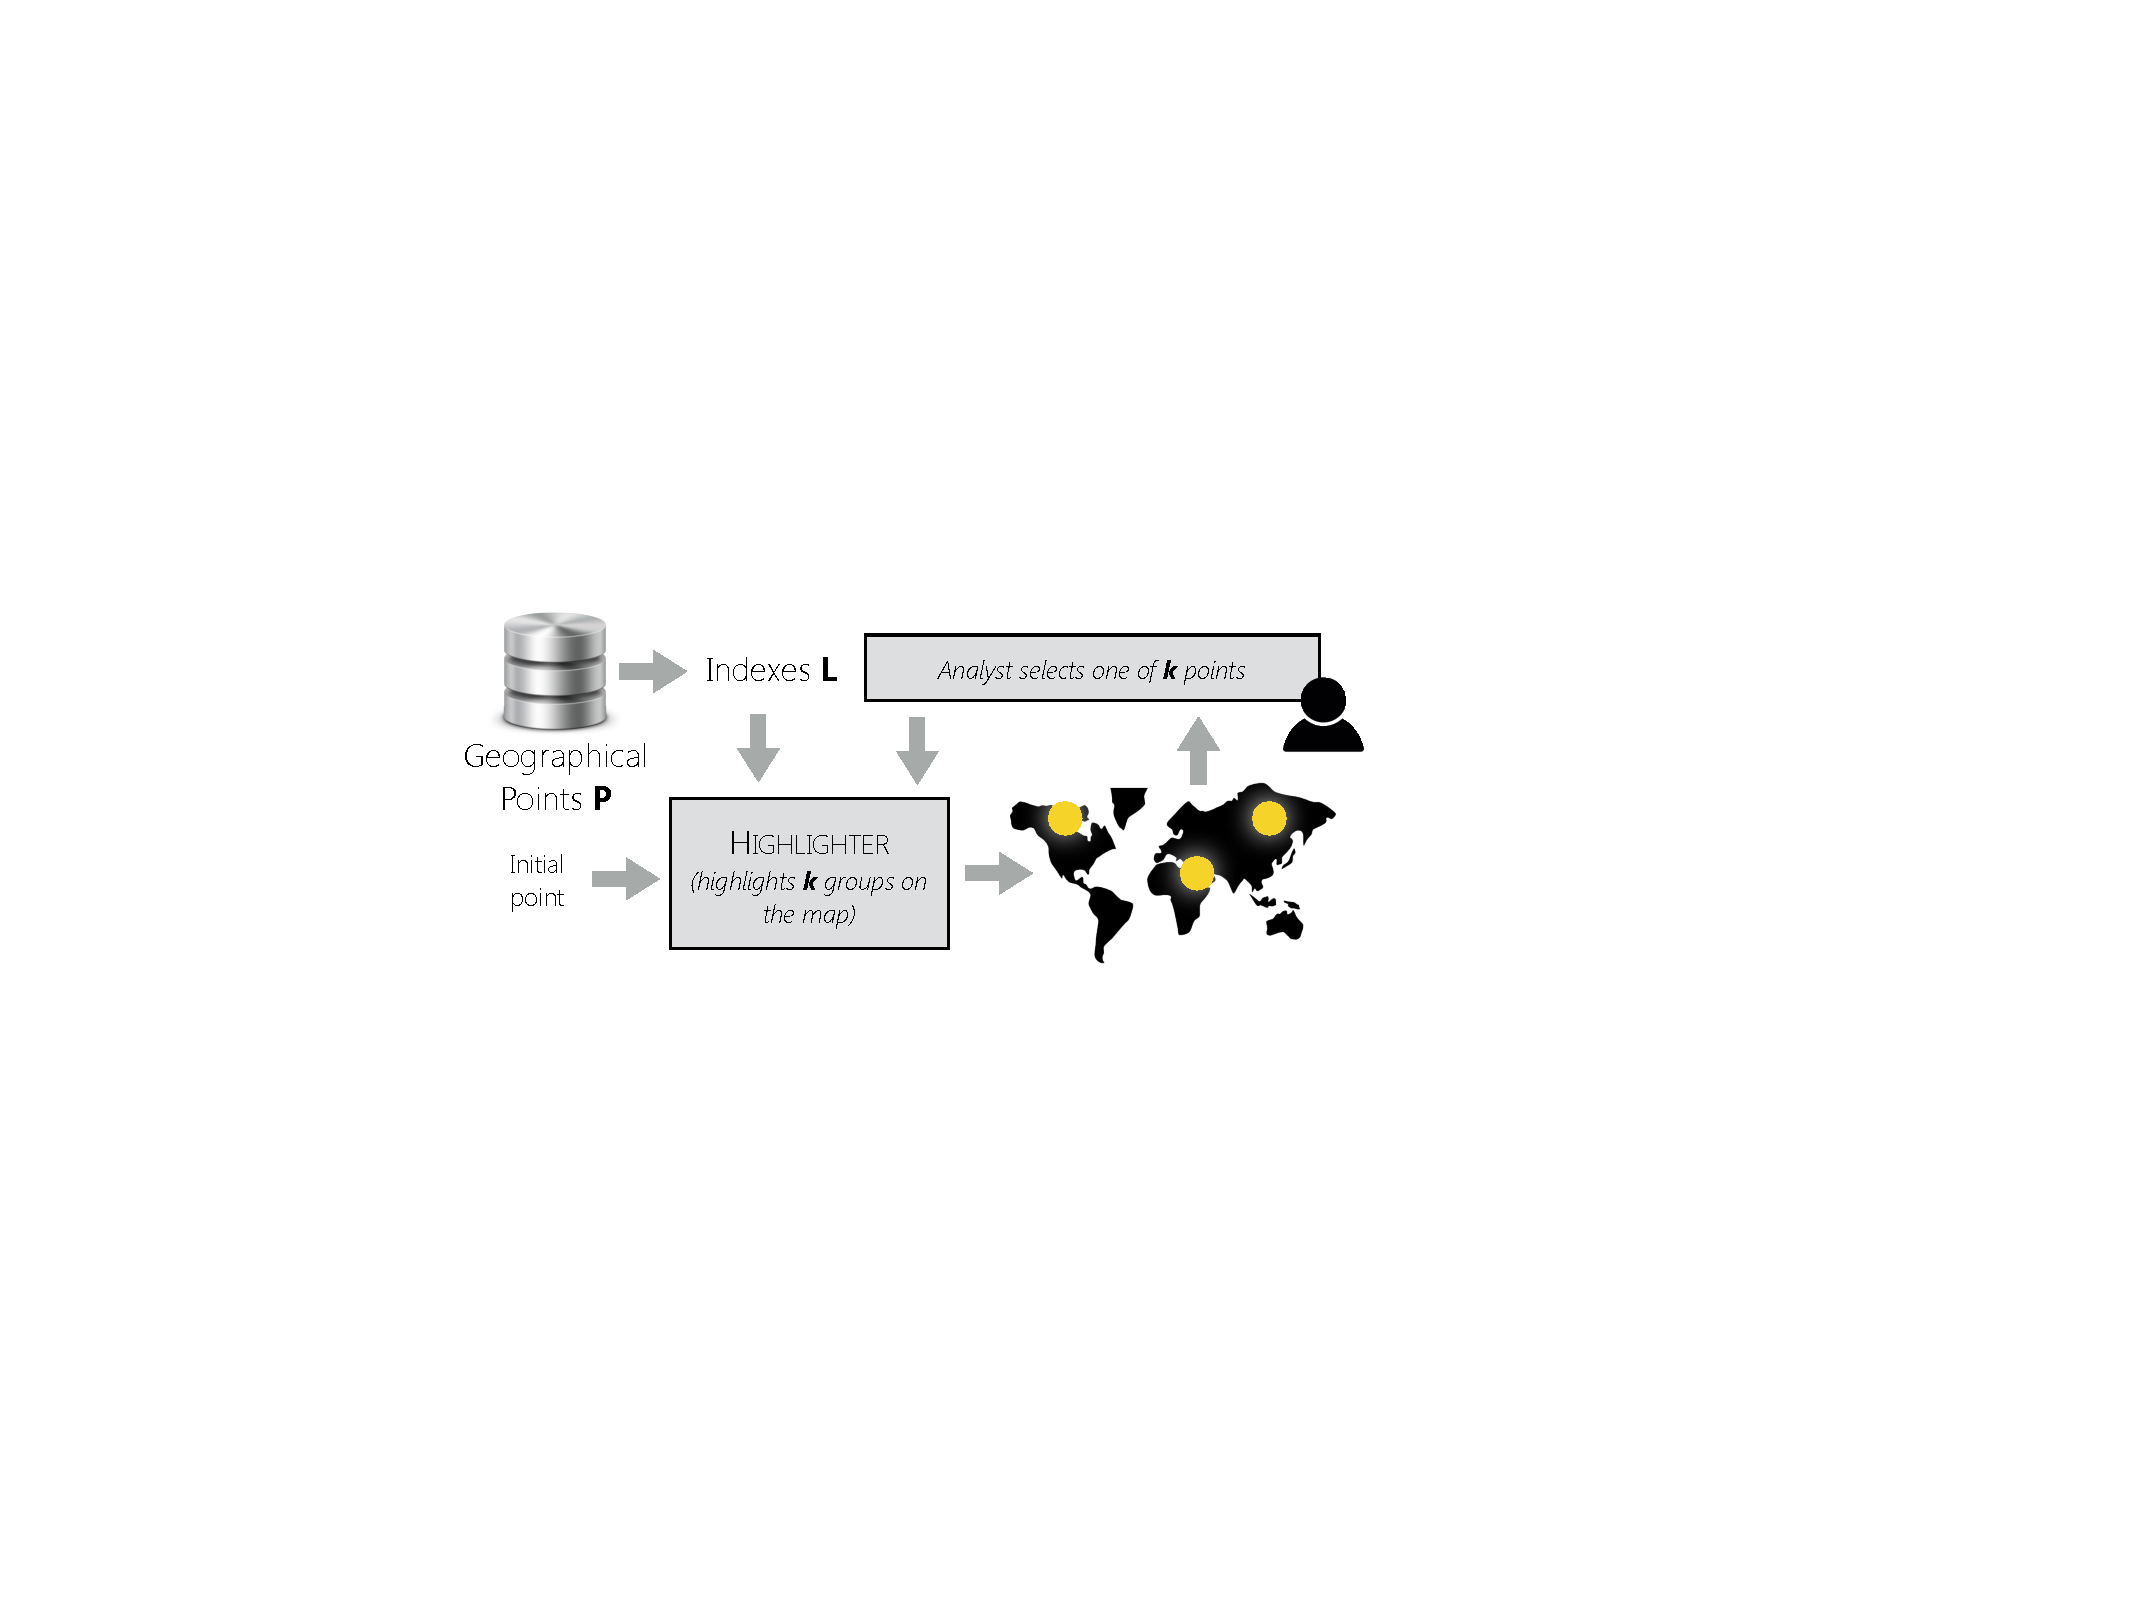
\includegraphics[width=\columnwidth]{figs/framework}
\caption{\framework\ Framework}
\label{fig:framework}
\vspace{-10pt}
\end{figure}

Traditionally, an exploratory analysis scenario on spatiotemporal data is described as follows: the analyst visualizes the data using an off-the-shelf product (e.g., Tableau\footnote{\it http://www.tableau.com},
% Exhibit\footnote{\it http://www.simile-widgets.org/exhibit/},
Spotfire\footnote{\it http://spotfire.tibco.com}). Then she looks at different parts of data for interesting patterns and trends. With the growing size of spatiotemporal datasets, this classical approach is not practical anymore: geographical points are scattered everywhere and the analyst cannot effectively observe insights.

To overcome this challenge, visualization environments offer a plethora of operations to filter out data. In practice, this doubles the problem: the analyst is left alone in a huge space of data and operations. 
In an exploratory context,
%Considering the exploratory context as a non-idempotent process\footnote{\it We call an interactive step as ``idempotent'' if it always follows the exact same steps.},
the principled challenge for the analyst is {\em ``what to see next''} during the analysis process. A {\em guidance mechanism} is necessary to point out potential future directions of analysis.

Given a geographical point of interest, the question is then how to recommend other points to be considered in future analysis steps in form of guidance. In this paper, we focus on one specific guidance approach, i.e., highlighting $k$-best points given a point of interest. Those $k$ points should have high quality. Quality is formulated as optimization of two dimensions: {\em relevance} and {\em diversity}. Optimizing relevance ensures that recommended points are in-line with what the analyst has already liked. Optimizing diversity results points which are as different as possible from each other and unveil different aspects of analysis. Example \ref{ex:flight} illustrates a common case in practice.

\begin{example}
\label{ex:flight}
Tiffany is a data scientist and is tasked to design a {\em chain marketing} strategy for a Peking Duck product whose headquarters is in New York. She already knows that the product has success in the local area. So she analyzes Yelp data\footnote{\it https://www.yelp.com/} (i.e., restaurant check-ins) to find out what other locations exhibit similar eating profiles as New York. She asks for $k$ geographical points which have relevant eating profile to New York and are the most diverse. Given $k=3$, Tiffany receives points from San Fransisco, Washington DC and Marlton, NJ. She selects Marlton due its proximity to reduce transportation costs. Then she asks for other 3 best points for Marlton. She can then make the city-to-city chain marketing strategy.
\end{example}

In this paper, we address the problem of guidance. Despite the great progress on spatiotemporal data analysis in recent years, we point out following challenges for guidance:
$i.$ {\em Genericness.} Considering the heterogeneous nature of spatiotemporal datasets, it is challenging to come up with a generic guidance approach which is independent of data type and distribution.
$ii.$ {\em Size}. The gigantic size of spatiotemporal datasets hinders its effective discovery. 
% The guidance approach should be able to provide a limited set of recommendations to overcome information overload.
$iii.$ {\em Efficiency.} Guidance should be done efficiently in consecutive steps, so that the train of the analyst's thoughts won't break. Despite progress in efficient spatiotemporal processing \cite{yu2015geospark}, sub-second interactivity is still missing.

% In terms of efficiency, {\sc GeoSpark} \cite{yu2015geospark} and {\sc SpatialHadoop} \cite{DBLP:conf/icde/EldawyM15} are two promising computing systems for efficient processing large-scale spatiotemporal data. Those systems can exploited as the backbone of \framework\ once large-scale data needs to be analyzed.

% \vspace{5pt}
% \noindent {\bf Related Work.}
There exist few instances of information-highlighting methods \cite{Liang2010,Robinson2011,wongsuphasawat2016voyager,willett2007scented}. However all these methods are {\em objective} and do not apply to the context of spatiotemporal guidance where user feedback is involved.  In terms of recommendation, few approaches focus on spatial dimension
% \cite{Levandoski:2012,Magdy2014,HendawiKRBTA15a,Bao2015,Magdy:2014}
\cite{Bao2015,Levandoski:2012}
while the context and result diversification are missing.
% In this paper, we addressed the problem of highlighting geographical points to
% guide analysts in consecutives steps. To the best of our knowledge, this is the
% first work which formulates the geo-highlighting problem for recommending on
% maps. However, our problem relates to a number of others as follows.     

% Visual Highlighting. There has been efforts to highlight some pieces of
% information in the huge heterogeneous data space so that the analyst can focus
% on important aspects \cite{}. Visual
% Story Construction is another domain of work \cite{} which
% consecutive analysis steps are created automatically. However, all such highlighting methods are objective and does not consider analyst
% interest. In GeoHiglight, we provide a simple yet effective feedback model which
% can feed the recommendation algorithm to produce relevant results to current
% investigations.        

% Some other works have exploited highlighting as a technique to synchronize
% coordinated views [CITE CROSSFILTER] or simplify complicated dataset
% visualizations \cite{Robinson2011,Alper:2011}. Also in \cite{Philipsen}
% different highlighting methods are compared in terms of efficiency and usefulness. Such methods are complementary to ours.     

% Spatiotemporal Interactive Analysis and Visualization. Being an interactive
% system, it should be efficient and capture user feedback and adapt the utility
% function. In terms of efficiency, SpatialHadoop \cite{} and GeoSpark \cite{}
% extend Hadoop and Spark ecosystems respectively to boost geographical
% computations and visualizations. Such systems can be exploited as the backbone
% of GeoHighlight once large-scale data needs to be analyzed.      

% In terms of feedback, many off-the-shelf products such as Tableau \cite{} and
% RapidMiner \cite{} are designed to visualize different kinds of datasets including
% spatiotemporal ones. However, ``recommendation'' is the missing component in
% most of such tools: providing a full package of operations and actions, the analyst
% may know what to do next. In such system, analysis is usually considered as a
% one-shot scenario, once in reality it happens in consecutive steps following
% user feedback.        

% Recommendation. There exist a huge body of work in recommendation
% \cite{Adomavicius:2005} for various domains and datasets. However, spatial
% dimension is still untouched and has not received a lot of attention. In
% \cite{ChirigatiDDF16} a prediction algorithm for urban data is introduced which operates offline. In
% \cite{Levandoski:2012,Magdy2014,HendawiKRBTA15a,Bao2015,Magdy:2014},
% recommendation and visualization tools are introduced in specific domains.
% However, most the such algorithms are not context-aware (based on user choices)
% and does not consider diversity as a global metric.    


% \vspace{5pt}
In this paper, we propose a generic interactive analysis approach for guiding analysts towards potential interesting points. The analyst considers the guidance and picks a direction for the next analysis iteration. 

% prune this
% \vspace{5pt}
% \noindent {\bf Outline.} in Section \ref{sec:data-model}, we present our data model. Then in Section \ref{sec:pb}, we formally define our problem. Section \ref{sec:algo} describes our solution for the guidance problem. We show a realistic application of our solution in Section \ref{sec:scenarios}. We present an extensive set of experiments in Section \ref{sec:exp}. A summary of related work is discussed in Section \ref{sec:rel}. Finally we conclude in Section \ref{sec:conc}.
\section{Data Model}\label{sec:data-model}
A spatiotemporal dataset contains a vast variety of datasets such as aviation, ground transportation (bike, taxi, renting-car, bus), urban data, geo-tagged social networks, crimes, events, etc. Intuitively, the common point between all those dataset is having {\em location} and {\em time} attributes. We propose a generic data model to capture all diverse aspects of such data. 

We consider a spatiotemporal database ${\cal D}$ consisting $\langle {\cal P}, {\cal A} \rangle$ where ${\cal P}$ is the set of
geographical points and ${\cal A}$ is the set of point attributes. For each $p \in {\cal P}$, we consider a tuple $<id, lat, lon, alt, t>$ where $id$ is the point identifier, $lat$, $lon$ and $alt$ denote $p$'s geographical coordinates (latitude, longitude and altitude respectively), and $t$ is the timestamp.

The set ${\cal A}_p$ contains attribute-values for $p$ over the schema of ${\cal A}$. For instance, on a bike-sharing dataset, ${\cal A}_p = \langle $ {\tt female}, {\tt young}, {\tt subscribed} $\rangle$ on the schema ${\cal A} = \langle$ {\tt gender}, {\tt age-category}, {\tt subscription} $\rangle$ denotes that $p$ is associated to a young female cyclist who is subscribed in the bike-sharing system. The set ${\cal A}$ is domain-dependent and defines the semantics of a spatiotemporal dataset. For instance, in case of a taxi dataset, ${\cal A} = \langle$ {\tt dropoff\_time}, {\tt price}, {\tt tip} $\rangle$, where for an aviation dataset, ${\cal A} = \langle$ {\tt aircraft\_type}, {\tt departure\_airport}, {\tt arrival\_airport} $\rangle$.

Some spatiotemporal datasets contain point-sets as entities, such as {\em trajectories} in transportation datasets and {\em regions} in urban or agriculture dataset. Although our generic data model only captures the finest granular concept (i.e., point), we define ${\cal S}$ containing point-sets. Each point-set $s \in {\cal S}$ is indeed a set of points where $s \subseteq {\cal P}$. For instance, in a taxi dataset, $s = [ p_1, p_2 \dots p_n ]$ shows a ride consisting $n$ points departing at $p_1$ and arriving at $p_n$.
\section{Problem Statement}
\label{sec:pb}
In an exploratory analysis context, the analyst does not necessarily know what to ask. She may have also a few knowledge about the spatiotemporal data and its attributes. Hence she usually needs to take iterative analysis steps to observe different aspects of data and ultimately land on a subset of interest. However, it is often cumbersome to choose what to analyze next. Because this choice is subjective and infeasible to capture with an unsupervised method.

In this paper, we address the problem of {\em generic guidance} in spatiotemporal data: ``what is the process of guiding analysts in iterative analysis steps on any spatiotemporal dataset?'' In other words, we are interested in an approach which highlights a set of $k$ points that the analyst should probably consider in the next analysis iteration. This should not be a heuristic-based data-dependent highlighting, but a {\em generic} approach which is applied on any spatiotemporal dataset. We describe the desiderata of generic guidance approach as follows.

\vspace{5pt}
\noindent {\bf Genericness.} The guidance component should be agnostic about the dataset type, attributes and distribution. In other words, no assumption should be taken into consideration in a guidance scenario.

\vspace{5pt}
\noindent {\bf Limited Options.} The set of $k$ highlighted points should not be very large so that the analyst may become overwhelmed and distracted with too many options \cite{miller1956human}.

\vspace{5pt}
\noindent {\bf Relevance.} The fundamental difference between highlighting and $k$-NN spatial queries \cite{aly2015spatial} is that in the former, the focus is not on $k$ points which are geographically close to a point of interest $p$, but the ones which have similar characteristics to $p$. In other words, we are interested in points which are {\em relevant} to a given point of interest. For instance, consider a taxi ride in New York for a young male customer for an itinerary of 10 miles and \$3 tip. In contrary to thousands of miles of geographical distance, the ride is very similar to another one in San Fransisco for a middle-age male customer for an itinerary of 8 miles and \$2.5 tip. Relevance is a pair-based metric which is associated to point characteristics. We define the relevance between a pair of points as follows.

\begin{definition}[Relevance]
Given two points $p_1$ and $p_2$ and their attribute values ${\cal A}_{p_1}$ and ${\cal A}_{p_2}$, the relevance between $p_1$ and $p_2$ is a value between $0$ and $1$ denoted as $\mathit{relevance}(p_1,p_2) = \mathit{average}_{a \in {\cal A}_{p_1} \cup {\cal A}_{p_2}}(\mathit{sim({\cal A}_{p_1}, {\cal A}_{p_2}, a)})$.
\label{def:rel}
\end{definition}

In Definition \ref{def:rel}, the similarity function $\mathit{sim}()$ can be any function such as Jaccard and Cosine. Each attribute can have its own similarity function (as string and integer attributes are compared differently). Then $\mathit{sim}()$ works as an overrding-function which maps provides encapsulated similarity computations for any type of attribute.

\vspace{5pt}
\noindent {\bf Diversity.} A guidance approach should also consider coverage of all points: $k$ given points should represent different regions so that the analyst can observe different aspects of her data and decide for the next analysis iteration. Hence, $k$ points should be {\em diverse}. Diversity is a set-based metric and is associated to geographical distance. We define this metric as follows.

\begin{definition}
Given a set of points $s = \{ p_1, p_2 \dots \}$, the diversity $s$ is defines as $\mathit{diversity}(s)$ $=$ $\mathit{average}_{\{p, p'\} \subseteq s | p \neq p' }$ $\mathit{distance}(p,p')$.
\label{def:divs}
\end{definition}

In Definition \ref{def:divs}, $\mathit{distance}(p,p')$ operates on geographical coordinates of $p$ and $p'$ and can be considered as any distance function of Chebyshev distance family such as Eucledian. However, as distance computations are done in {\em spherical space} using latitude, longitude and altitude, hence the most logical distance function to employ is Harvestine. The Harvestinve distance of two geographical points $p$ and $p'$ is calculated as shown in Equation \ref{eq:harvestine}.

\begin{dmath}
\label{eq:harvestine}
distance(p,p') = [ acos(cos(p_{lat}) . cos(p'_{lat}) . cos(p_{lng}) . cos(p'_{lng})\\ + cos(p_{lat}) . sin(p'_{lat}). cos(p_{lng}) . sin(p'_{lng}) + sin(p_{lat}) . sin(p'_{lat})) ] \times earth\_radius
\end{dmath}

Following aforementioned desiderata, we forumlate highlighting as an optimization-based problem where we optimize diversity and respect a bound on relevance.

\begin{problem}[GeoHighlight]
\label{pb:geoh}
Given an input point $p$ and $\sigma$, the problem is to return $k$-relevant points to $p$ denoted $S_p$ where $|S_p| = k$ and $\forall p' \in S_p, \mathit{relevance}(p,p') \geq \sigma$ and $\mathit{diversity}(S_p)$ is maximized.
\end{problem}

Problem \ref{pb:geoh} is hard due to the huge space of spatiotemporal data: for any given point $p$, an exhaustive search over all other points is necessary to find $k$ points with maximal relevance. Moreover, the problem expresses interest in obtaining high quality points in two dimensions at the same time (relevance and diverse) which makes the problem even harder.

% behrooz: talk about quality earlier
\section{Algorithm}\label{sec:algorithm}

Assume n points are currently shown on the map. The analysis clicks on one point p1. p1 has a set of attributes associated to it in A. Based on this set of attributes, a similarity can be measured between p1 and ant other n points. It can be for instance Cosine or Euclidean. Then the ordered list specifies the most similar points to p1. Basically we can highlight first k points in this ordered list. However, these top-k points may be too much close to each other so that it doesn’t give that much insights to the analyst.

We sacrifice similarity to gain diversity. In a greedy approach, we investigate on the k+1, k+2 … points in the ordered list and verify if the diversity increases. We can define diversity as the average/sum of distances between points. We consider a time limit (user given) and during this time limit, we try to move towards more diversity. Once the time limit expires, we show final k points.

This idea is based on \cite{Omidvar-Tehrani:2015}.
\section{Illustrative Scenario}\label{sec:scenarios}
We illustrate an application of \framework\ in a realistic scenario for New York taxi dataset\footnote{\it https://data.cityofnewyork.us/view/gn7m-em8n}. This dataset has been frequently exploited for urban analysis
% \cite{ferreira2013visual,DBLP:journals/debu/FreireCVZ16}.
(e.g., \cite{DBLP:journals/debu/FreireCVZ16}).
The dataset contains 173,179,759 records of taxi trips and 18 attributes such as pickup and dropoff date/time, passenger count and trip distance.
% The dataset size is 27.9 GB with informations of trips from 2014.
The scenario illustrates how an analyst can achieve an exploratory analysis goal. We preprocessed the original dataset and considered a subset of 100K unique points for the sake of clarity of results. We employ {\sc Highlighter} (Algorithm \ref{algo:geoh}) with following parameters: $\sigma = 0.7$, $k = 5$ and $tlimit = 200ms$.

\begin{figure}
  \centering
  
\includegraphics[width=\columnwidth]{figs/placeholder}
\caption{Application of \framework\ on New York Taxi dataset}
\label{fig:app}
\end{figure}

% \vspace{5pt}
Consider Lucas, a data scientist whose task is to optimize New York taxi trips. Focusing on cab-idle locations, he wants to discover which neighborhoods work the best for which drivers to increase the overall availability. Also, he wants to discover how drivers should choose their next cab-idle station to be more available. Lucas employs \framework\ and follows a case-by-case inspection as his analysis methodology by analyzing and learning from historical data.

% coordinates of first point picked: lat, long: 40.757555, -73.988832. Point ID-1274, equivalent to 270 W 43rd St, New York, NY 10036, EUA. Next to Times Square.
% coordinates of the second point: lat, long: 40.789358,-73.970172000000005. Point ID-968, equivalent to Columbus Avenue, New York, NY, EUA.
%  coordinates of the third point: lat, long: 40.717531999999999,-74.010260000000002. Point ID-192, equivalent to 183 Duane Street, New York, NY 10013, EUA
He begins the analysis by selecting a point from the most crowded region in New York, i.e., Times Square. The point depicts a drop-off at {\em 270 West 43rd Street} on January 9, 2014 at 10PM. {\sc Highlighter} then provides $5$ relevant points to the selected point (Figure \ref{fig:app}).
% These highlights show similar points to the selection in other neighborhoods of the region.
Among 5 highlighted points, Lucas selects the 3rd one, i.e., a pick-up at {\em Columbus Avenue} near Central Park occurred approximately at the same time of the first selection. This pick-up has a potential to enchain with the first choice (i.e., a drop-off) to engage the driver in a larger distance.

In the next step, {\sc Highlighter} shows 5 other points relevant to the new selection. Lucas looks for a good drop-off point which is in a neighborhood of the previous selection as the cab-idle station. Lucas selects the second highlighted point at {\em 183 Duane Street} at \colorred{[time?]} as other highlights are around airport and train stations which have less taxi requests in the afternoon. This selection contributes to the heavy cab request in Manhattan island at that time of the day. 

% The result of similarity for all two executions of the algorithm for the Lucas problem, considering $k = 5$ and $\sigma = 0.2$, was approximately, \textit{0.72}.
\section{Experiments}
\label{sec:exp}
We evaluate the efficiency and usefulness of {\sc GeoHighlight} in an extensive set of experiments. We consider two types of experiments: first, a performance study to measure the influence of {\em similarity}, size constraint $k$, and $tlimit$ on execution time, and second, a user study to evaluate how efficient analysts can gain insights in our framework.

\vspace{5pt}
\noindent {\bf Experiment Settings.} Unless otherwise states, we set $k = 5$, $\sigma = 0.4$, and $tlimit = 200ms$. We use New York dataset for our experiments. All experiments are implemented in Python (functionality) and JavaScript (visualization) on a 2.4GHz Intel Core i5 machine with an 8GB main memory, running OS X 10.9.2.

\begin{figure}
  \centering
  
\includegraphics[width=\columnwidth]{figs/placeholder}
\caption{Performance Evaluation}
\label{fig:performance}
\end{figure}

\vspace{5pt}
\noindent {\bf Performance Study.} {\sc GeoHighlight} is designed for exploratory context where interactivity is a need. The best-effort greedy approach of {\sc Highlighter} (Algorithm \ref{algo:geoh}) guarantees to return the best possible results within a time limit. We consider a large time limit in order evaluate the effect of similarity and size constraint $k$ on execution time. Figure \ref{fig:performance} illustrates the results.

Figure \ref{fig:performance} left illustrates the effect of size constraint by varying $k$ from $2$ to $500$.

\vspace{5pt}
\noindent {\bf User Study.}
\section{Related Work}
\label{sec:rel}

% In this paper, we addressed the problem of highlighting geographical points to
% guide analysts in consecutives steps. To the best of our knowledge, this is the
% first work which formulates the geo-highlighting problem for recommending on
% maps. However, our problem relates to a number of others as follows.     

% Visual Highlighting. There has been efforts to highlight some pieces of
% information in the huge heterogeneous data space so that the analyst can focus
% on important aspects \cite{Liang2010,Lohmann:2012,Robinson2011}. Visual
% Story Construction is another domain of work \cite{Segel:2010,Samet:2014} which
% consecutive analysis steps are created automatically. However, all such highlighting methods are objective and does not consider analyst
% interest. In GeoHiglight, we provide a simple yet effective feedback model which
% can feed the recommendation algorithm to produce relevant results to current
% investigations.        

% Some other works have exploited highlighting as a technique to synchronize
% coordinated views [CITE CROSSFILTER] or simplify complicated dataset
% visualizations \cite{Robinson2011,Alper:2011}. Also in \cite{Philipsen}
% different highlighting methods are compared in terms of efficiency and usefulness. Such methods are complementary to ours.     

% Spatiotemporal Interactive Analysis and Visualization. Being an interactive
% system, it should be efficient and capture user feedback and adapt the utility
% function. In terms of efficiency, SpatialHadoop \cite{} and GeoSpark \cite{}
% extend Hadoop and Spark ecosystems respectively to boost geographical
% computations and visualizations. Such systems can be exploited as the backbone
% of GeoHighlight once large-scale data needs to be analyzed.      

% In terms of feedback, many off-the-shelf products such as Tableau \cite{} and
% RapidMiner \cite{} are designed to visualize different kinds of datasets including
% spatiotemporal ones. However, ``recommendation'' is the missing component in
% most of such tools: providing a full package of operations and actions, the analyst
% may know what to do next. In such system, analysis is usually considered as a
% one-shot scenario, once in reality it happens in consecutive steps following
% user feedback.        

% Recommendation. There exist a huge body of work in recommendation
% \cite{Adomavicius:2005} for various domains and datasets. However, spatial
% dimension is still untouched and has not received a lot of attention. In
% \cite{ChirigatiDDF16} a prediction algorithm for urban data is introduced which operates offline. In
% \cite{Levandoski:2012,Magdy2014,HendawiKRBTA15a,Bao2015,Magdy:2014},
% recommendation and visualization tools are introduced in specific domains.
% However, most the such algorithms are not context-aware (based on user choices)
% and does not consider diversity as a global metric.    

\section{Conclusion}
\label{sec:conc}



\bibliographystyle{abbrv}
\bibliography{main} 

\end{document}
